% !TeX root = ../document_main.tex
% ============================================================
% 12. DEPLOYMENT STRATEGY
% ============================================================
\begin{sectionintro}{12}{Deployment Strategy}{
  \begin{itemize}[leftmargin=1.5em]
    \item Multi-service container orchestration with Docker Compose
    \item Security-critical Vault-first secrets bootstrapping workflow
    \item Isolated virtual bridge networks and fail-closed security posture
    \item Air-gapped self-hosted packaging with a Bubble Tea TUI installer
    \item Automated CI/CD validation pipelines with GitHub Actions
    \item Observability stack using OpenTelemetry, Prometheus, Jaeger, and Loki
  \end{itemize}
}
A secure, resilient, and reproducible deployment strategy is a fundamental requirement for a Zero-Trust Database Access Gateway. Because the \texttt{zGate} platform stands as the exclusive security boundary between developers and production database systems, its deployment infrastructure must itself embody zero-trust principles: minimal attack surfaces, isolated network topologies, fail-closed transport mechanisms, and strict secrets separation.

This chapter details the deployment architecture of the \texttt{zGate} ecosystem. We examine the containerized multi-service orchestration model, environment isolation strategies, and the security-critical ``Vault-first'' secrets bootstrapping workflow. Additionally, we document the self-hosted air-gapped packaging strategy, the automated GitHub Actions CI/CD validation pipelines, and the operational observability architecture that integrates OpenTelemetry, Prometheus, Jaeger, and Loki.
\end{sectionintro}
\label{ch:deployment_strategy}

% ============================================================
\section{Orchestration and Deployment Topology}
% ============================================================
The \texttt{zGate} platform is deployed as a containerized microservices stack. By utilizing containerization, the platform achieves operational consistency across local development, cloud staging, and physical on-premises environments.

\subsection{Multi-Service Container Stack}
The complete deployment topology is defined in a centralized Docker Compose configuration (\texttt{docker-compose.yml}), orchestrating nine independent, tightly coupled services. These services cooperate over an isolated virtual bridge network (\texttt{zgate-net}) to isolate traffic between the control plane, data plane, and management plane:

\begin{figure}[H]
    \centering
    \begin{tikzpicture}[
        node distance=1.8cm,
        box/.style={rectangle, rounded corners, minimum width=2.8cm, minimum height=1.0cm, align=center, draw=black, fill=blue!10, font=\footnotesize},
        netline/.style={draw=black, line width=1.5pt, dashed},
        arrow/.style={thick,->,>=stealth}
    ]
        % Isolated network line
        \draw[netline] (-6,0) -- (6,0) node[right] {\textbf{\texttt{zgate-net}}};

        % Services
        \node (vault) [box, fill=purple!20, above of=start, yshift=2.0cm, xshift=-4.5cm] {\textbf{Vault}\\(Secrets Hub)};
        \node (mysql) [box, fill=orange!20, above of=start, yshift=2.0cm, xshift=-1.5cm] {\textbf{MySQL}\\(Control Store)};
        \node (keycloak) [box, fill=red!20, above of=start, yshift=2.0cm, xshift=1.5cm] {\textbf{Keycloak}\\(SSO IdP)};
        \node (tsql) [box, fill=teal!20, above of=start, yshift=2.0cm, xshift=4.5cm] {\textbf{T-SQL Sidecar}\\(gRPC Parser)};

        \node (server) [box, fill=blue!20, below of=start, yshift=-1.5cm, xshift=-3cm] {\textbf{zGate Server}\\(Proxy Gateway)};
        \node (webui) [box, fill=cyan!20, below of=start, yshift=-1.5cm, xshift=0cm] {\textbf{zGate WebUI}\\(Admin Portal)};
        \node (ai) [box, fill=green!20, below of=start, yshift=-1.5cm, xshift=3cm] {\textbf{zGate AI}\\(ML Anomaly)};

        \node (otel) [box, fill=gray!25, below of=server, yshift=-0.8cm, xshift=3cm] {\textbf{OTel Collector}\\(Telemetry Ingress)};

        % Connections to network
        \draw[thick] (vault.south) -- (-4.5,0);
        \draw[thick] (mysql.south) -- (-1.5,0);
        \draw[thick] (keycloak.south) -- (1.5,0);
        \draw[thick] (tsql.south) -- (4.5,0);
        \draw[thick] (server.north) -- (-3,0);
        \draw[thick] (webui.north) -- (0,0);
        \draw[thick] (ai.north) -- (3,0);

        % Dynamic communication
        \draw[arrow, <->] (server.east) -- (webui.west);
        \draw[arrow, ->] (server.south) -| (otel.north);
        \draw[arrow, ->] (webui.south) -- (otel.north);
        \draw[arrow, ->] (ai.south) -| (otel.north);
    \end{tikzpicture}
    \caption{Logical Deployment Network Topology}
    \label{fig:deployment-network}
\end{figure}

The specific role and configuration properties of each service in the stack are as follows:
\begin{enumerate}
    \item \textbf{\texttt{vault}} (\texttt{hashicorp/vault:1.15}): The secure secrets storage vault. It runs in a fail-closed configuration, storing encrypted DSN secrets, JWT keys, and TLS CA credentials. It communicates over port \texttt{8200}.
    \item \textbf{\texttt{mysql}} (\texttt{mysql:8}): The persistent control-plane database. It holds user rosters, role-to-permission mappings, system configurations, compliance definitions, and in-progress session metadata. Crucially, the control-plane data is encrypted at rest at the field level, and it is isolated from the downstream database targets.
    \item \textbf{\texttt{keycloak}} (\texttt{zgate-keycloak-vault}): The federated Identity Provider. It implements OpenID Connect (OIDC) authentication flows for single sign-on (SSO) and client credential verification, publishing its JWKS endpoint at port \texttt{8180}.
    \item \textbf{\texttt{keycloak-init}} (\texttt{curlimages/curl}): A transient, one-shot bootstrap container. It waits for Keycloak to boot, retrieves administrative passwords from Vault, and executes API calls to configure security settings (such as disabling HTTPS enforcement for the internal proxy network or syncing Master realm credentials).
    \item \textbf{\texttt{tsql-parser}}: A high-performance gRPC parsing sidecar. The zGate Go server delegates Transact-SQL (T-SQL) query parsing to this container over a local Unix domain socket mounted at \path{/var/run/zgate/tsql.sock}.
    \item \textbf{\texttt{zgate-server}} (\texttt{ghcr.io/zgatehq/zgate-server}): The core database wire-protocol gateway and REST API. It exposes proxy ports for database protocols (\texttt{9000} for MySQL, \texttt{9001} for PostgreSQL, and \texttt{9002} for MS SQL Server) and the administrative REST endpoints (\texttt{8080}).
    \item \textbf{\texttt{zgate-webui}} (\texttt{ghcr.io/zgatehq/zgate-webui}): The Next.js 15 administrative portal. It provides visual access control management, audit logging dashboards, and real-time session tracking, running on host port \texttt{3000}.
    \item \textbf{\texttt{zgate-ai}} (\texttt{ghcr.io/zgatehq/zgate-ai}): The machine-learning anomaly detection and PII column-masking service. It runs on port \texttt{8001} and periodically retrains Isolation Forest models using SQL trace outputs.
    \item \textbf{\texttt{otel-collector}} (\texttt{otel/opentelemetry-collector}): The standards-compliant telemetry aggregator. It accepts traces, metrics, and logs over OTLP/gRPC and forwards them to Jaeger, Prometheus, and Loki.
\end{enumerate}

\subsection{Vault-First Bootstrapping and AppRole Integration}
To enforce zero-trust posture, the system implements a \textbf{``Vault-first''} dependency model. No component in the stack may contain hardcoded plaintext secrets in its environment definitions or image configurations. Instead, container boot sequences are split into two sequential phases:

\begin{enumerate}
    \item \textbf{Identity Verification Phase:} At startup, each service container receives its unique HashiCorp Vault AppRole credentials via environment variables: a non-secret \texttt{VAULT\_ROLE\_ID} and a single-use, short-lived \texttt{VAULT\_SECRET\_ID}.
    \item \textbf{Secret Retrieval Phase:} The container entrypoint executes a login against the Vault API endpoint (\texttt{/v1/auth/approle/login}) using the AppRole credentials to obtain a temporary \texttt{VAULT\_TOKEN}. It then uses this token to retrieve database passwords, encryption keys, and private certificates from Vault paths (e.g., \texttt{secret/data/zgate/mysql}).
\end{enumerate}

If Vault is unreachable, or if the provided \texttt{VAULT\_SECRET\_ID} has expired or has already been used (enforcing single-use semantics), the entrypoint script fails immediately, and the container process exits. This prevents services from booting in an unconfigured or fallback state, satisfying the strict ``fail-closed'' requirement.

% ============================================================
\section{Environment Strategy}
% ============================================================
The deployment workflow partitions configurations across three distinct environments (Development, Staging, and Production) to maintain operational isolation and enforce the principle of least privilege.

\subsection{Environment Partitioning}
Table~\ref{tab:environments} outlines the infrastructure configurations, credentials, and verification requirements across the environment lifecycle:

\begin{table}[H]
\centering
\caption{Environment Lifecycle Separation}
\label{tab:environments}
\resizebox{\textwidth}{!}{%
\begin{tabular}{|l|l|l|l|}
\hline
\textbf{Parameter} & \textbf{Development} & \textbf{Staging} & \textbf{Production} \\
\hline
\textbf{Orchestrator} & Docker Compose & Docker Compose / Kubernetes & Bare-Metal / Enterprise VMs \\
\textbf{Vault Status} & Development Mode & Shared Vault Instance & Shamir-Sealed (5/3 Threshold) \\
\textbf{Identity Store} & Local Mock / SQLite & Keycloak Staging Realm & Keycloak SSO + Active Directory \\
\textbf{TLS Enforcement} & Plain TCP Allowed & Strict Server TLS & Mutual TLS (mTLS) Enforced \\
\textbf{Log Level} & \texttt{debug} & \texttt{info} & \texttt{warn} / \texttt{error} \\
\textbf{Audit Target} & Standard Output & Local File Rotation & Immutable Syslog / Elasticsearch \\
\hline
\end{tabular}%
}
\end{table}

\subsection{Orchestration Script (\texttt{start.sh})}
To automate deployment and minimize manual configuration drift, the repository provides an idempotent bash orchestrator script (\texttt{start.sh}). When executed, the orchestrator performs the following tasks:

\begin{enumerate}
    \item \textbf{Secrets Generation:} Generates cryptographically secure keys (e.g., a 64-character hex key for \texttt{ZGATE\_STORE\_KEY}, random passwords for MySQL administrative accounts, and Keycloak client secrets).
    \item \textbf{Internal CA and Certificate Bootstrapping:} Generates an internal root CA certificate using ECDSA P-256 and issues TLS server certificates for the database proxy ports and administrative REST APIs.
    \item \textbf{Vault Initialization and Shamir Unsealing:} Initializes Vault and returns five Shamir unseal keys and an initial root token. The orchestrator unseals Vault using three of the five keys (satisfying the 5/3 threshold).
    \item \textbf{AppRole Provisioning:} Enters Vault, mounts the AppRole authentication engine, defines security policies for each service container, and provisions the necessary \texttt{role\_id} and \texttt{secret\_id} pairs.
    \item \textbf{Config Seeding:} Writes the generated passwords and certificate PEMs into Vault's KV-v2 engine.
    \item \textbf{Environment Variable Assembly:} Assembles the local environment file (\texttt{.env}) containing the service AppRole credentials and starts the Docker Compose stack using the profiles \texttt{infra} and \texttt{apps}.
\end{enumerate}

% ============================================================
\section{Self-Hosted and Air-Gapped Strategy}
% ============================================================
Enterprise customers operating in highly sensitive sectors (such as finance, healthcare, or government) require the database proxy to run in isolated, air-gapped on-premises data centers without internet connectivity. The \texttt{zGate} ecosystem provides a dedicated self-hosting package to support this model.

\subsection{Air-Gapped Package Composition}
The offline distribution is compiled as a self-contained tarball archive (\texttt{zgate-selfhost.tar.gz}) containing:
\begin{itemize}
    \item Compressed OCI container images for all nine stack services.
    \item The local \texttt{docker-compose.yml} configuration.
    \item Pre-rendered administrative themes and Keycloak realm configurations.
    \item An interactive Go-based installer executable (\texttt{install-zgate}).
\end{itemize}

The container images are pre-packaged on an internet-connected build machine using the script \texttt{export-images.sh}. This script pulls the official production container tags from the GitHub Container Registry (GHCR), retags them as local offline images (e.g., \texttt{zgate-server:offline}), and exports them to a unified tar archive:

\begin{lstlisting}[style=code, caption=Offline Image Packaging Script (\texttt{export-images.sh})]
#!/bin/bash
set -euo pipefail

IMAGES=(
  "ghcr.io/zgatehq/zgate-server:latest"
  "ghcr.io/zgatehq/zgate-webui:latest"
  "ghcr.io/zgatehq/zgate-ai:latest"
  "hashicorp/vault:1.15"
  "mysql:8"
)

OUTPUT_DIR="./images"
mkdir -p "$OUTPUT_DIR"

for img in "${IMAGES[@]}"; do
  echo "Pulling $img..."
  docker pull "$img"
  filename=$(echo "$img" | sed 's|/|_|g' | sed 's|:|__|g')
  echo "Exporting to $OUTPUT_DIR/${filename}.tar..."
  docker save "$img" -o "$OUTPUT_DIR/${filename}.tar"
done
tar -czf zgate-images.tar.gz -C "$OUTPUT_DIR" .
\end{lstlisting}

\subsection{Interactive Bubble Tea Installer}
In an air-gapped environment, operators interact with the installation bundle using the \texttt{install-zgate} executable. The installer is built in Go using the Bubble Tea TUI framework, providing a step-by-step terminal interface that coordinates system preparation:

\begin{figure}[H]
    \centering
    \begin{mdframed}[backgroundcolor=gray!10, linecolor=gray!40, linewidth=2pt]
        \begin{verbatim}
+-----------------------------------------------------------+
|                   zGate Offline Installer                 |
+-----------------------------------------------------------+
|                                                           |
|  [x] Verify Docker & Docker Compose                       |
|  [x] Validate License File (zgate.lic)                    |
|  [>] Load Container Images (zgate-images.tar.gz)          |
|  [ ] Bootstrap Local HashiCorp Vault                      |
|  [ ] Generate mTLS Trust Store and CA                     |
|  [ ] Seed Control-Plane Schema (MySQL)                    |
|                                                           |
|  Progress: [=====================>           ] 55%        |
|  Status: Loading image zgate-server:offline...            |
+-----------------------------------------------------------+
        \end{verbatim}
    \end{mdframed}
    \caption{Conceptual Bubble Tea TUI Installer Flow}
    \label{fig:tui-installer}
\end{figure}

The installer automates the import process by executing \texttt{docker load} on all packaged image tarballs, verifying system requirements, and invoking the local secrets initialization routine without calling external endpoints.

\subsection{Hardware-Bound License Validation}
To prevent unauthorized replication of the platform within private clouds, the installation executable enforces a hardware-bound licensing model. The process operates as follows:

\begin{enumerate}
    \item \textbf{Hardware Fingerprinting:} The installer reads host machine identifiers (e.g., the system UUID from DMI tables, CPU serial numbers, and motherboard identifiers).
    \item \textbf{Hardware Hash Generation:} The collected values are normalized and hashed using SHA-256 to produce a unique \textbf{Hardware ID}.
    \item \textbf{License File Verification:} The installer reads the local license file (\texttt{zgate.lic}). The file contains the buyer's metadata, expiration date, authorized database count, and the signed Hardware ID. The signature is verified using a hardcoded public ECDSA key.
    \item \textbf{Hardware Matching:} If the signature is valid, the installer generates the local Hardware ID and matches it against the value embedded in the license. If they do not match, the installation aborts, enforcing host-level copy protection.
\end{enumerate}

\subsection{Hardened Enforced Image Variants}
For maximum security in self-hosted deployments, the CI/CD pipeline builds two distinct variants of the server and web dashboard images: standard and \textbf{enforced}.

The enforced variants (tagged as \texttt{:enforced}) contain binary compilations where critical security boundaries (e.g., license validation routines, administrative portal lockdown modes, and Keycloak realm settings) are hardcoded into the binaries using Go compiler link flags (\texttt{-ldflags}) and Next.js build-time variables. Because these settings are baked directly into the executable binary code rather than being read from mutable environment variables or external configuration files, they cannot be manipulated or bypassed by an operator with host-level root access, mitigating insider tampering risks.

% ============================================================
\section{CI/CD Pipeline Strategy}
% ============================================================
The transition of code from Git commits to production container registries is automated via GitHub Actions workflows. The pipelines enforce code quality, run unit/integration test suites, and perform security vulnerability scanning before generating OCI-compliant artifacts.

\subsection{Server CI/CD Workflow (\texttt{docker.yml})}
The server pipeline compiles the Go gateway and packages the OCI container images. The logical flow is detailed in Figure~\ref{fig:cicd-server-pipeline}:

\begin{figure}[H]
    \centering
    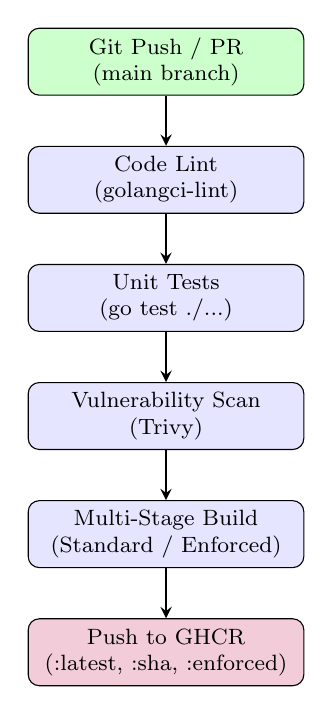
\begin{tikzpicture}[
        node distance=1.5cm,
        box/.style={rectangle, rounded corners, minimum width=3.5cm, minimum height=0.85cm, align=center, draw=black, fill=blue!10, font=\footnotesize},
        arrow/.style={thick,->,>=stealth}
    ]
        \node (trigger) [box, fill=green!20] {Git Push / PR\\(main branch)};
        \node (lint) [box, below of=trigger] {Code Lint\\(golangci-lint)};
        \node (test) [box, below of=lint] {Unit Tests\\(go test ./...)};
        \node (scan) [box, below of=test] {Vulnerability Scan\\(Trivy)};
        \node (build) [box, below of=scan] {Multi-Stage Build\\(Standard / Enforced)};
        \node (push) [box, below of=build, fill=purple!20] {Push to GHCR\\(:latest, :sha, :enforced)};

        \draw[arrow] (trigger) -- (lint);
        \draw[arrow] (lint) -- (test);
        \draw[arrow] (test) -- (scan);
        \draw[arrow] (scan) -- (build);
        \draw[arrow] (build) -- (push);
    \end{tikzpicture}
    \caption{Server CI/CD Build Pipeline Flow}
    \label{fig:cicd-server-pipeline}
\end{figure}

The server Dockerfile utilizes a multi-stage compilation to keep the production runtime small. The first stage uses a \texttt{golang:1.26-alpine} builder to compile the statically linked binary, and the final production stage uses a minimal \texttt{gcr.io/distroless/base} image, which contains no shell, package manager, or command-line utilities, reducing the container's attack surface.

\subsection{WebUI CI/CD Workflow}
The frontend pipeline builds and audits the Next.js administration portal:
\begin{enumerate}
    \item \textbf{Dependency Resolution:} Uses \texttt{pnpm} to install packages, caching the store to accelerate build times.
    \item \textbf{Syntax and Formatting Linting:} Runs \texttt{pnpm lint} and type-checks the source files using TypeScript compiler (\texttt{tsc}).
    \item \textbf{Test Suite Execution:} Runs Vitest tests with a strict 60\% code coverage threshold.
    \item \textbf{Production Standalone Build:} Compiles the Next.js application using the \texttt{standalone} output configuration. This configures Next.js to trace and copy only the necessary files to a self-contained directory, excluding the bloated \texttt{node\_modules} folder.
    \item \textbf{Containerization:} Packages the standalone build into a production Docker image and pushes it to GHCR.
\end{enumerate}

\subsection{CLI Cross-Compilation and Release Workflow}
Because the command-line client is an executable distributed directly to developer endpoints, its release pipeline must support multiple operating systems and CPU architectures. The workflow, triggered by Git semantic version tags (e.g., \texttt{v1.2.3}), is managed by GoReleaser:

\begin{table}[H]
\centering
\caption{CLI Cross-Compilation Release Matrix}
\label{tab:cli-matrix}
\begin{tabular}{|l|l|l|}
\hline
\textbf{Target OS} & \textbf{Architectures} & \textbf{Binary Output Format} \\
\hline
Linux & \texttt{amd64}, \texttt{arm64} & \texttt{zgate-cli\_linux\_amd64.tar.gz} \\
macOS & \texttt{amd64}, \texttt{arm64} (Apple Silicon) & \texttt{zgate-cli\_darwin\_all.zip} \\
Windows & \texttt{amd64} & \texttt{zgate-cli\_windows\_amd64.zip} \\
\hline
\end{tabular}
\end{table}

The release pipeline executes the following sequence:
\begin{enumerate}
    \item \textbf{Ldflags Injection:} Injects the tag version, Git commit SHA, and compilation timestamp into the Cobra CLI configuration at compile time:
    \begin{verbatim}
go build -ldflags "-X main.version=v1.2.3 -X main.commit=abcdefg" -o zgate .
    \end{verbatim}
    \item \textbf{Artifact Signing:} Generates SHA-256 checksums for each archive and signs them using Cosign with the project's release key.
    \item \textbf{Release Publication:} Uploads the compiled zip and tarball archives to the GitHub Releases page.
    \item \textbf{Repository Dispatch Trigger:} Triggers a workflow dispatch event to the main server repository (\texttt{zGate}). The server workflow downloads the newly released CLI binaries and embeds them inside the server's static asset directory (\path{/static/cli/}). This ensures that the server's download endpoint (\texttt{GET /api/cli/download}) always serves the latest matching client version.
\end{enumerate}

% ============================================================
\section{Observability, Monitoring, and Operations}
% ============================================================
Operating a security-critical gateway in production requires real-time observability to detect policy violations, connection latency spikes, and system failures.

\subsection{OpenTelemetry Collector Architecture}
The observability stack is designed around OpenTelemetry. Rather than requiring containers to send telemetry directly to monitoring systems, each service exports data to a local OpenTelemetry Collector daemon over the network using the open-source OTLP protocol.

The OTel Collector (\texttt{otel-collector-config.yaml}) acts as a buffer. It processes the incoming signals, filters out internal metrics, and distributes them to the backend storage engines:

\begin{figure}[H]
    \centering
    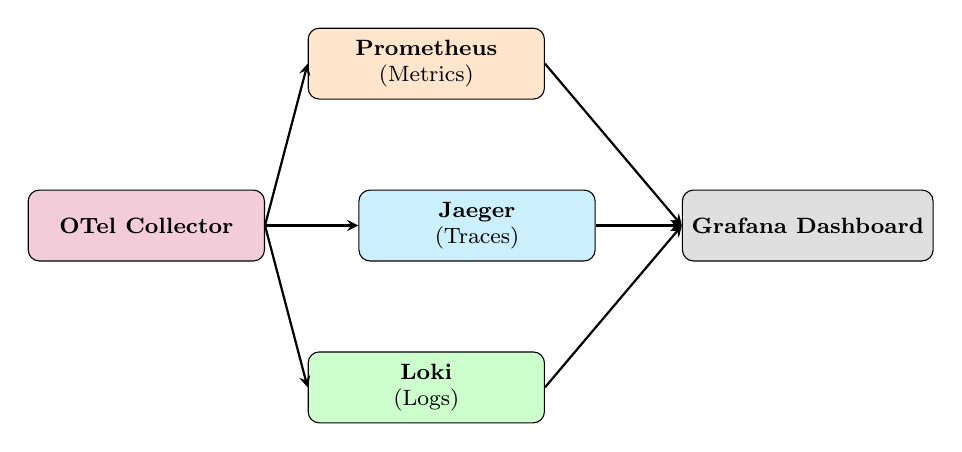
\begin{tikzpicture}[
        node distance=2.2cm,
        box/.style={rectangle, rounded corners, minimum width=3.0cm, minimum height=0.9cm, align=center, draw=black, fill=blue!10, font=\footnotesize},
        arrow/.style={thick,->,>=stealth}
    ]
        % Collector
        \node (collector) [box, fill=purple!20] {\textbf{OTel Collector}};

        % Backends
        \node (prometheus) [box, fill=orange!20, above right of=collector, xshift=2.0cm, yshift=0.5cm] {\textbf{Prometheus}\\(Metrics)};
        \node (jaeger) [box, fill=cyan!20, right of=collector, xshift=2.0cm] {\textbf{Jaeger}\\(Traces)};
        \node (loki) [box, fill=green!20, below right of=collector, xshift=2.0cm, yshift=-0.5cm] {\textbf{Loki}\\(Logs)};

        % Frontends
        \node (grafana) [box, fill=gray!25, right of=jaeger, xshift=2.0cm] {\textbf{Grafana Dashboard}};

        % Connections
        \draw[arrow] (collector.east) -- (prometheus.west);
        \draw[arrow] (collector.east) -- (jaeger.west);
        \draw[arrow] (collector.east) -- (loki.west);

        \draw[arrow] (prometheus.east) -- (grafana.west);
        \draw[arrow] (jaeger.east) -- (grafana.west);
        \draw[arrow] (loki.east) -- (grafana.west);
    \end{tikzpicture}
    \caption{Telemetry Routing and Visualization Architecture}
    \label{fig:observability-architecture}
\end{figure}

\subsection{Monitoring Stack Integration}
The individual telemetry stores collect specialized performance data:
\begin{itemize}
    \item \textbf{Prometheus (Metrics):} Collects resource usage (CPU and memory consumption), connection metrics (active database sessions, network packet sizes), and proxy statistics (query rate limits, count of queries blocked by safety templates).
    \item \textbf{Jaeger (Distributed Tracing):} Traces the path of connection requests and administrative API operations. This allows operators to visualize latency bottlenecks, showing exactly how long a request takes within the OIDC authentication check, the Vault credential lookup, the gRPC query parser, the AI masking engine, and the physical database.
    \item \textbf{Loki (Log Aggregation):} Aggregates the standard output logs of all services. It uses labels (such as \texttt{container\_name}) to support querying and log correlation.
\end{itemize}

\subsection{Internal PKI and Certificate Revocation Cache}
Transport security is managed by the internal CA (\texttt{CAManager}). When a client connects using mutual TLS, the Go server's connection verification callback (\texttt{VerifyConnection}) validates the client certificate's trust chain.

To handle revocation without the latency overhead of checking external OCSP responders or CRL files on every connection, the server maintains an in-memory \textbf{Revocation Cache}. The cache is synchronized with the control-plane database's \texttt{certificates} table. When an administrator revokes a user's certificate or service account credential, the cache is updated. Subsequent connections using that certificate fingerprint are immediately rejected during the TLS handshake, terminating the session before it reaches the SQL parser.

\subsection{Fail-Closed Posture and Security Checklist}
The deployment configuration maintains a fail-closed posture. If the telemetry agent detects that the logging backend is full, or that Vault has entered a sealed state, the system automatically triggers a shutdown of active proxy listeners. This prevents transactions from proceeding without an active audit trail.

Table~\ref{tab:sec-checklist} summarizes the operational checklist required to maintain a secure deployment in production:

\begin{table}[H]
\centering
\caption{Production Security Settings Checklist}
\label{tab:sec-checklist}
\resizebox{\textwidth}{!}{%
\begin{tabular}{|l|l|l|}
\hline
\textbf{Configuration Item} & \textbf{Value} & \textbf{Security Objective} \\
\hline
\texttt{ENFORCE\_MTLS} & \texttt{true} & Prevent plain TCP credential exchanges \\
\texttt{VAULT\_ADDR} & \texttt{https://vault:8200} & Encrypt secrets traffic in transit \\
\texttt{ZGATE\_LOG\_LEVEL} & \texttt{warn} / \texttt{error} & Prevent credential leaks in debug logs \\
\texttt{ZGATE\_ALLOW\_TICKET\_REUSE} & \texttt{false} & Prevent ticket hijacking and replay attacks \\
\texttt{PROXY\_HANDSHAKE\_LIMIT} & \texttt{256} & Mitigate DoS attacks on proxy listener ports \\
\texttt{ANOMALY\_CONTAMINATION} & \texttt{0.02} & Tune anomaly engine sensitivity \\
\hline
\end{tabular}%
}
\end{table}
